\documentclass[12pt,a4paper]{article}
\usepackage{graphicx} % Required for inserting images
\setlength{\topmargin}{0.0in}
\setlength{\oddsidemargin}{0.33in}
\setlength{\textheight}{9.0in}
\setlength{\textwidth}{6.0in}
\renewcommand{\baselinestretch}{1.25}


\usepackage{hyperref}
% \usepackage[utf8]{inputenc}
% \usepackage[T1]{fontenc}
\usepackage{float}
\usepackage{enumitem}
\usepackage{amsmath}
\usepackage{amssymb}
\usepackage{amsthm}
\usepackage{tikz}
\usepackage{amsfonts}
\usepackage{graphicx}
\usepackage{subcaption}
\usepackage{caption}
\newcommand{\dv}[2]{\frac{\mathrm{d} #1}{\mathrm{d} #2}}
\usepackage{caption}
\captionsetup[figure]{font=small} 
% \captionsetup[table]{font=small}
\usepackage[capitalize,nameinlink]{cleveref}
\usepackage{mathtools}
\newcommand{\defeq}{\vcentcolon=}
\newcommand{\eqdef}{=\vcentcolon}



\newtheoremstyle{boldthm}
  {3pt}        % space above
  {3pt}        % space below
  {\itshape}   % body font
  {}           % indent
  {\bfseries}  % theorem head font
  {.}          % punctuation
  {.5em}       % space after theorem head
  {\thmname{#1}\thmnumber{ #2}\thmnote{ \textbf{(#3)}}}

\newtheoremstyle{bolddefn}
  {3pt}
  {3pt}
  {\itshape} 
  {}
  {\bfseries}
  {.}
  {.5em}
  {\thmname{#1}\thmnumber{ #2}\thmnote{ \textbf{(#3)}}}


\theoremstyle{boldthm}
\newtheorem{theorem}{Theorem}[section]
\newtheorem{corollary}[theorem]{Corollary}
\newtheorem{lemma}[theorem]{Lemma}
\newtheorem{proposition}[theorem]{Proposition}

\theoremstyle{bolddefn}
\newtheorem{definition}[theorem]{Definition}
\newtheorem{example}[theorem]{Example}
\newtheorem{remark}[theorem]{Remark}

% Define environments
% \newtheorem{theorem}{Theorem}
% \newtheorem{definition}{Definition}
% \newtheorem{lemma}{Lemma}
% \newtheorem{corollary}{Corollary}


\title{Some Background Notes}
\author{Maggie McCarthy}
\date{May 2026}

\begin{document}

\maketitle

% \textbf{TOMORROW - Normal operators, spectra and pseudo spectra results, finish Umberto's second lecture, prep for meeting, review Matt's preliminaries.}

In the following, the numbers in parentheses refer to the relevant page number in Kreyszig's functional analysis text \cite{krey}. 

\section{Functional Analysis Review}

% Unless otherwise stated, $X$ and $Y$ denote two Banach spaces (complete normed spaces) with the corresponding norms $\| \cdot \|_X$ and $\| \cdot \|_Y,$ respectively. Furthermore, the domain, range, and nullspace of an operator $T$ are denoted by $D(T),$ $R(T),$ and $N(T),$ respectively.

\subsection{Linear Operators}

Let $L(X, Y)$ denote the set of linear operators from the vector space $X$ to the vector space $Y.$ A linear operator is defined as follows:
\begin{definition}[{Linear operator \cite[2.6-1]{krey}}]
    Let $X$ and $Y$ be vector spaces over the same field. Let $D(T) \subset X.$
   An operator $T : D(T) \rightarrow Z$ is called linear if it satisfies  $T(ax+by) = aTx + bTy$ for all $x, y \in D(T)$ and for any scalars $a, b.$ 
\end{definition}
% Going forward, we will denote the set of linear operators from $X$ to $Y$ by $L(X, Y).$ 

Assuming that $T \in L(X, Y)$ is injective, there exists a mapping $T^{-1}: R(T) \rightarrow D(T)$ that sends every $y \in R(T)$ to the unique $x \in D(T)$ for which $Tx = y.$ Some useful properties of $T^{-1}$ are given in the following theorem:

\begin{theorem}[{Inverse operator \cite[2.6-10]{krey}}] \label{inv}
Let $X$ and $Y$ be vector spaces over the same field. Let $T : D(T) \rightarrow Y$ be a linear operator with $D(T) \subset X$ and $R(T) \subset Y.$ Then 
\begin{enumerate}
    \item $T^{-1} : R(T) \rightarrow D(T)$ exists if and only if $T$ is injective.
    \item If $T^{-1}$ exists it is a linear operator.
    \item If $\text{dim}(D(T)) = n < \infty$ and $T^{-1}$ exists then $\text{dim}(R(T)) = \text{dim}(D(T)).$
\end{enumerate}
    
\end{theorem}


Bounded, compact, and closed linear operators will be used throughout. A bounded linear operator is defined as follows:
\begin{definition}[{Bounded operator \cite[2.7-1]{krey}}] 
    Let $X$ and $Y$ be normed spaces. $T \in L(X, Y)$ is a bounded linear operator if there exists a $c>0$ such that $\|Tx\|_Y \le c \|x\|_X$ for all $x \in D(T).$ 
\end{definition}
We use $B(X,Y)$ to denote the set of all bounded linear operators from $X$ to $Y,$ equipped with the norm 
\begin{equation}
    \|T\|_{B(X, Y)} = \sup_{x \in X} \frac{\| Tx \|_Y}{\|x\|_X}.
\end{equation}

Similarly, we will use $K(X, Y)$ to denote the set of compact linear operators from $X$ to $Y.$ A compact linear operator is defined as follows:

\begin{definition}[{Compact linear operator \cite[8.1-1]{krey}}] 
Let $X$ and $Y$ be normed spaces. $T \in L(X, Y)$ is a compact linear operator if for every bounded subset $M$ of $X,$ the image $T(M)$ is relatively compact, that is, the closure $\overline{T(M)}$ is compact. Equivalently, $T$ is compact if and only if it maps every bounded sequence $\{x_n\}_{n \in \mathbb{N}}$ in $X$ onto a sequence  $\{Tx_n\}_{n \in \mathbb{N}}$ in $Y$ that has a convergent subsequence.
\end{definition}
Every compact linear operator is bounded. Thus, $K(X, Y) \subset B(X, Y)$ (406). The following theorem describes the situation in which the composition of a bounded linear operator with a compact operator is compact \cite{umberto}.

\begin{theorem}
   Consider $S \in B(X, X)$ and $T \in K(X, Y).$ The operator $TS$ is compact, i.e., $TS \in K(X, Y).$  
\end{theorem}

\begin{proof}
    Let $\{x_n\}_{n \in \mathbb{N}}$ be a bounded sequence in $X.$ Since $S \in B(X, Y),$ $\| S x_n \| \le \| S \|_{B(X, Y)} \| x_n \|_{X}$ for all $n \in \mathbb{N}.$ Since $\{x_n\}_{n \in \mathbb{N}}$ is a bounded sequence and $S$ is a bounded operator, we can say  $\|S x_n \| < \infty.$ Thus, $\{S x_n\}_{n \in \mathbb{N}}$ is a bounded sequence in $X.$  Since $T$ is compact, applying $T$ to a bounded sequence in $X$ yields a sequence in $Y$ with a convergent subsequence. Thus, $T\{S x_n\}_{n \in \mathbb{N}} = (TS)\{ x_n\}_{n \in \mathbb{N}}$ has a convergent sequence in $Y$ and $TS \in K(X, Y).$
\end{proof}

In spectral theory, we often consider closed operators, which are defined as follows:
\begin{definition}[{Closed linear operator \cite[4.13-1]{krey}}] 
     Let $X$ and $Y$ be normed spaces.  $T \in L(X, Y)$ is called a closed linear operator if its graph,
    \begin{equation}
        G(T) = \{(x, y) \mid x \in D(T), y = Tx\},
    \end{equation}
    is closed in the normed space $X \times Y,$ where the two algebraic operations of the vector space $X \times Y$ are defined as usual, and the norm is defined by $\|(x, y)\|_{X \times Y} = \|x\|_{X} + \|y \|_{Y}.$ 
\end{definition}
Alternatively, closed operators can be defined using the following theorem:
\begin{theorem}[{Closed linear operator \cite[4.13-3]{krey}}]\label{closed}
     Let $X$ and $Y$ be normed spaces. $T \in L(X, Y)$ is a closed linear operator if and only if it has the following property: whenever $\{x_n\}_{n \in \mathbb{N}}$ is a sequence in $D(T)$ such that $x_n \rightarrow x$ and $Tx_n \rightarrow y,$ then $x \in D(T)$ and $Tx = y.$
\end{theorem}
Going forward, $C(X, Y)$ will denote the set of closed linear operators from $X$ to $Y.$ To close out this section, we recall the Closed Graph Theorem:
\begin{theorem}[{Closed Graph Theorem \cite[4.13-2]{krey}}]  \label{CGT}
    Let $X$ and $Y$ be Banach spaces and $T \in C(X, Y)$ with $D(T) \subset X.$ If $D(T)$ is closed in $X,$ then $T$ is bounded. 
\end{theorem}
% When $A$ is closed and invertible, so is $A^{-1}$ (the graph of $A^{-1}$ is the `flip' of the graph of $A$). 

\subsection{A Survey of Results}

Next, we collect several important results that will be useful in the proofs that follow. We first consider the Open Mapping Theorem and the Bounded Inverse Theorem, whose proofs are given in \cite{krey}.

% Finally, we define an open mapping as follows
\begin{definition}[{Open mapping \cite[4.12-1]{krey}}] 
    Let $X$ and $Y$ be two metric spaces. Then $T : D(T) \rightarrow Y,$ where $D(T) \subset X,$ is called an open mapping if for every open set in $D(T),$ the image is an open set in $Y.$
\end{definition}

\begin{theorem}[{Open Mapping Theorem \cite[4.12-2]{krey}}] 
    Let $X$ and $Y$ be two Banach spaces, i.e., complete normed spaces. $T \in B(X, Y)$ is an open mapping.
\end{theorem}

\begin{theorem}[{Bounded Inverse Theorem \cite[4.12-2]{krey}}]  \label{BIT}
     Let $X$ and $Y$ be two Banach spaces. If $T \in B(X, Y)$ is bijective, then $T^{-1}$ is bounded. 
\end{theorem}


Often, we will make use of the Neumann series, defined in the following theorem:

\begin{theorem}[{Neumann Series \cite[7.3-1]{krey}}]  \label{neum}
    Let $T \in B(X, X),$ where $X$ is a Banach space. If $\|T\|_{B(X, X)} < 1,$ then $(I - T)^{-1}$ exists as a bounded linear operator on the whole space $X.$ Furthermore, 
    \begin{equation}
        (I - T)^{-1} = \sum_{j=1}^{\infty} T^j = I + T + T^2 + \dots,
    \end{equation}
    where the series on the right is convergent in the norm on $B(X, X).$
\end{theorem}


Finally, we recall two results that will be useful in understanding the spectra of compact operators. 
\begin{theorem}[Riesz's Lemma \cite{umberto}] \label{RL}
    Let $W$ and $X$ be normed spaces where $W$ is a closed proper subset of $X.$ Then for every $\epsilon > 0,$ there exists a $x \in X$ such that $\|x\|_X = 1$ and $\text{dist}(x, W) \ge 1-\epsilon.$
\end{theorem}

\begin{corollary}[{Riesz's Ball Theorem \cite[2.5-5]{krey}}] \label{ball}
    Let $X$ be a normed linear space and $B$ be the closed unit ball in $X.$ If $X$ is finite dimensional then $B$ is compact. If $X$ is infinite-dimensional, then $B$ is never compact.
\end{corollary}


\subsection{Banach and Hilbert Adjoints}

Recall that a \textit{linear functional} is a linear operator whose domain is a vector space and whose range is the corresponding scalar field. Similarly, a linear functional is bounded when it is a bounded linear operator. 

Before defining the Adjoint of a linear operator, we first recall the definition of a dual space.
\begin{definition}[{Dual space \cite[2.10-3]{krey}}] 
    Let $X$ be a normed space. The set of all bounded linear functionals on X is the normed space $X^*,$ referred to as the dual space of $X.$ The dual space is equipped with the following norm:
    \begin{equation}
        \| f \| = \sup_{\substack{x \in X \\ \|x\|_X =1}} | f(x) |. 
    \end{equation}
\end{definition} 

% \subsubsection{Banach Adjoint}

Let $ X$ and $Y$ be two Banach spaces and let $T \in B(X, Y).$ We use $\langle x_*, x \rangle_{X^*, X}$ to denote the action of the element $x_* \in X^*$ on an element $x \in X.$ In other words, $\langle x_*, x \rangle_{X^*, X}$ denotes the application of the functional $x_*$ to $x.$ 

 For any $y^* \in Y^*$ and $x \in X,$ define the functional $G_{y_*}(x) = \langle y_*, Tx \rangle_{Y^*, Y}.$ From the linearity and boundedness of $T$ and $y_*,$ we find that $G_{y_*}$ is a bounded linear functional on $X,$ and is thus an element of $X^*$.
 % This functional is linear because both $T$ and $y_*$ are linear. This functional is bounded because $T$ and $y_*$ are bounded, and
% \begin{equation}
%     |G_{y_*} | = | \langle y_*, Tx \rangle_{Y^*, Y} | \le \| y_* \|_{Y^*} \| T \|_{B(X, Y)} \| x \|_{X}.
% \end{equation}
% Thus, $G_{y_*}$ belongs to $X^*.$ 
Using this functional, we define the Banach adjoint as follows:
\begin{definition}[Banach Adjoint \cite{umberto}] \label{BA}
    Let $X$ and $Y$ be Banach spaces and $T \in B(X, Y).$ The Banach adjoint of $T,$ denoted $T^*,$ is the operator in $B(Y^*, X^*)$ that maps $y_* \in Y^*$ to $G_{y_*},$ where $G_{y_*}(x) = \langle y_*, T_x \rangle_{Y^*, Y}.$
\end{definition}

Let $H$ denote a Hilbert space, i.e., a complete inner product space, with norm $\|\cdot\|_H$ and inner product $(\cdot, \cdot)_H.$ To define the Hilbert adjoint, we first recall the following result:
\begin{theorem}[{Riesz's Representation Theorem \cite[3.8-1]{krey}}]  \label{RR}
    Given any $h_* \in H^*,$ there exists a unique $h \in H$ such that $\langle h_*, k \rangle_{H^*, H} = (h, k)_H$ for all $k \in H.$ Furthermore, $\| h \|_H = \| h \|_{H^*}.$
\end{theorem}
Using this result, we define the Riesz map of $H$ as follows:
\begin{definition}[Riesz map \cite{umberto}]
    Following the notation in Theorem \ref{RR}, we define the Riesz map of $H$ as the map $R_H : H^* \rightarrow H$ that maps $h_*$ to $h.$ This map is bijective. 
\end{definition}

Using the Riesz map, the Hilbert adjoint\footnote{To compare the Banach and the Hilbert adjoints, consider the examples presented in Umberto's first lecture \cite{umberto}. These are worked out in detail in my written notes.} is defined as follows:
\begin{definition}[Hilbert Adjoint \cite{umberto}] \label{HA}
    Let $H_1$ and $H_2$ be two Hilbert spaces. Consider $T \in B(H_1, H_2)$ and its Banach adjoint $T^* \in B(H_2^*, H_1^*).$ The Hilbert adjoint is the operator $T' : H_2 \rightarrow H_1$ that maps $x \in H_2$  to $R_{H_1} T^* R_{H_2}^{-1} x \in H_1,$ where $R_{H_1}$ and $R_{H_2}$ are the Riesz maps for $H_1$ and $H_2,$ respectively.
\end{definition}
Alternatively, we can define the Hilbert adjoint with the following result
\begin{theorem} [Hilbert Adjoint \cite{umberto}] 
     Let $H_1$ and $H_2$ be two Hilbert spaces and $T \in B(H_1, H_2).$ The Hilbert adjoint, $T' : H_2 \rightarrow H_1$ can be defined as the operator in $B(H_2, H_1)$ that satisfies $(Th, x)_{H_2} = (h, T'x)_{H_1}$ for all $(h, x)$ in $H_1 \times H_2.$
\end{theorem}
\begin{proof}
    For $h \in H_1$ and $x \in H_2,$ we have
    \begin{equation}
    \begin{aligned}
        (h,T'x)_{H_1}
        &= (h,R_{H_1}T^*R_{H_2}^{-1}x)_{H_1}
        && \text{by Definition \ref{HA}} \\
        &= \langle T^*R_{H_2}^{-1}x,h\rangle_{H_1^*,H_1}
        && \text{by the definition of } R_{H_1} \\
        &= \langle R_{H_2}^{-1}x,Th\rangle_{H_2^*,H_2}
        && \text{by Definition \ref{BA}} \\
        &= (Th,x)_{H_2}
        && \text{by the definition of } R_{H_2},
    \end{aligned}
    \end{equation}
as desired.
\end{proof}
% \begin{proof}
%     Using Definition \ref{HA}, 
%     \begin{equation}
%     \begin{aligned}
%         (h, T'x)_{H_1} &= (h, R_{H_1} T^* R_{H_2}^{-1} x)_{H_1}.
%     \end{aligned}
%     \end{equation}
%     Using the definition of the Riesz map $R_{H_1},$
%         \begin{equation}
%     \begin{aligned}
%         (h, T'x)_{H_1} &= (h, R_{H_1} T^* R_{H_2}^{-1} x)_{H_1} \\
%         &= \langle T^* R_{H_2}^{-1} x, h \rangle_{H_1^*, H_1}.
%     \end{aligned}
%     \end{equation}
%     Using the definition of the Banach adjoint in Definition \ref{BA}, we have 
%     \begin{equation}
%     \begin{aligned}
%         (h, T'x)_{H_1} &= (h, R_{H_1} T^* R_{H_2}^{-1} x)_{H_1} \\
%         &= \langle T^* R_{H_2}^{-1} x, h \rangle_{H_1^*, H_1}\\
%         & = \langle R_{H_2}^{-1} x, Th \rangle_{H_2^*, H_2}.
%     \end{aligned}
%     \end{equation}
%     Finally, using the definition of the Riesz map $R_{H_2}$ we obtain the desired result:
%         \begin{equation}
%     \begin{aligned}
%         (h, T'x)_{H_1} &= (h, R_{H_1} T^* R_{H_2}^{-1} x)_{H_1} \\
%         &= \langle T^* R_{H_2}^{-1} x, h \rangle_{H_1^*, H_1}\\
%         & = \langle R_{H_2}^{-1} x, Th \rangle_{H_2^*, H_2}\\
%         &= (Th, x)_{H_2}.
%     \end{aligned}
%     \end{equation}
    
% \end{proof}

We now list some general properties of the Hilbert adjoint that are used frequently in applications. The proofs of these results can be found in \cite{krey}.  
\begin{theorem}[{Properties of Hilbert adjoint \cite[3.9-4]{krey}}] 
    Let $H_1$ and $H_2$ be two Hilbert spaces. Consider $S \in B(H_1, H_2)$ and $T \in B(H_1, H_2).$ Then for any $\alpha \in \mathbb{C},$ we have 
\begin{enumerate}[label=(\alph*)]
    \item For any $x \in H_1$ and $y \in H_2,$ $(T'y, x)_{H_1} = (y, Tx)_{H_2}$
    \item $(S + T)' = S' + T'$
    \item $(\alpha T)' = \bar{\alpha} T'$
    \item (T')' = T 
    \item $\| T' T \|_{B(H_1, H_1)} = \| T T' \|_{B(H_2, H_2)} = \| T \|_{B(H_1, H_2)}^2 $
    \item $T'T = 0 \iff T = 0$
    \item When $H_1 = H_2$ we have $(ST)' = T'S'.$
\end{enumerate}
\end{theorem}

    



\subsection{Self-Adjoint, Unitary, and Normal Operators}

Let $H$ be a Hilbert space, and let $T \in B(H, H)$ be an endomorphism. $T$ is \textit{self-adjoint} if $T' = T.$ Furthermore, if $T \in B(H, H)$ is self-adjoint and invertible, $T^{-1} \in B(H, H)$ is self-adjoint as well \cite{krey}. 

% We caution the reader that when $T$ is not bounded, $(Tx, y)_H = (x, T'y)_H$ does not guarentee that $T$ is self-adjoint. In particular, if $T=T'$ the operator is said to be formally adjoint. For $T$ to be self-adjoint, we need $T = T'$ and $D(T) = D(T').$

If $T \in B(H, H)$ satisfies $T'T = TT'$, it is called normal. Notice that when $T$ is self-adjoint, it is \textit{normal}. However, a normal operator need not be self-adjoint. $T \in B(H, H)$ is said to be \textit{unitary} if $T$ is bijective and $T' = T^{-1}.$ If $T$ is unitary, then  $T$ is normal. As before, the converse is generally not true \cite{krey}. 

We describe some criteria for self-adjointness in the following theorem:
\begin{theorem}[{Self-adjointness \cite[3.10-3]{krey}}] 
    Let $H$ be a Hilbert space and $T \in B(H, H).$ Then 
    \begin{enumerate}[label=(\alph*)]
        \item If $T$ is self-adjoint, $(Tx, x)_H$ is real for all $x \in H.$
        \item If $H$ is complex and $(Tx, x)_H$ is real for all $x \in H,$ then $T$ is self-adjoint.
    \end{enumerate}
\end{theorem}





\subsection{Beginner Spectral Theory}

In this section, we review some basic concepts from spectral theory, one of the main branches of modern functional analysis. We begin with a review of spectral theory in finite dimensions. 

\subsubsection{Spectral Theory in Finite Dimensions}

Let $W$ be an $n$-dimensional normed space, where $n < \infty.$ Let $T \in L(W, W)$ be represented by the matrix $A \in \mathbb{C}^{n \times n}.$ 

\begin{definition}[{Eigenvalues, eigenvectors, eigenspaces, spectrum, resolvent set \cite[7.1.1]{krey}}] \label{finite eig}
    Consider the following equation
    \begin{equation} \label{eig eq}
        Ax = \lambda x.
    \end{equation}
    An eigenvalue of $A$ is a $\lambda \in \mathbb{C}$ such that \eqref{eig eq} has a nontrivial solution, $x \ne 0$. This nontrivial solution is called an eigenvector of $A$ corresponding to $\lambda.$ The set of all eigenvectors corresponding to $\lambda,$ together with the zero vector, forms a vector subspace of $W$ called the eigenspace of $A$ corresponding to $\lambda.$ The set of all the eigenvalues of $A$ is called the spectrum of $A,$ denoted $\Gamma(A).$ Its complement is called the resolvent set, denoted $\rho(A) = \mathbb{C} \setminus \Gamma(A).$
\end{definition}

To find the eigenvalues and corresponding eigenvectors of $A,$ we rewrite \eqref{eig eq} as 
\begin{equation} \label{char}
    (A-\lambda I) x = 0,
\end{equation}
where $I$ is the identity matrix in $\mathbb{C}^{n\times n}.$ For this equation to have a nonzero solution, we require that the determinant of $(A-\lambda I)$ is zero. Thus, the eigenvalues of $A$ can be found by solving $\det (A-\lambda I) = 0,$ which is called the \textit{characteristic polynomial} of $A.$ Once the eigenvalues have been computed, the corresponding eigenvectors are found by solving \eqref{char}.


Each choice of basis for $W$ corresponds to a different matrix $A \in \mathbb{C}^{n \times n}$ used to represent $T \in L(W, W).$
Although the matrix representation of $T$ is not unique, all choices of $A$ have the same eigenvalues (366). Thus, the eigenvalues of $T$ are the eigenvalues of $A.$ Similarly, the spectrum and resolvent set of $A$ are the spectrum and resolvent set of $T.$ 





\subsubsection{Spectral Theory in Infinite Dimensions}


Let $X \ne \{0\}$ be a normed space and $T \in L(X, X).$ With $T$ we associate the operator $T_z = T - zI,$ where $z \in \mathbb{C}$ and $I$ is the identity operator on $D(T) \subset W.$ If $T_z$ has an inverse, we call it the resolvent operator of $T,$ denoted $R_T(z) = T_z^{-1} = (T-zI)^{-1}.$  

% By Theorem \ref{inv}, $R_T(z)$ is a linear operator
% any properties of $T_z$ and $R_T(z)$ depend on $z.$ Spectral theory is concerned with these properties.


 To dive deeper into spectral theory, we will need to define its most fundamental concepts, namely, the regular values of $T$, the resolvent set of $T$, and the spectrum of $T.$

 \begin{definition}[{Regular value \cite[7.2-1]{krey}}] \label{reg}
 Let $T \in L(X, X).$ A regular value of $T$ is a $z \in \mathbb{C}$ such that 
\begin{enumerate}[label=(R\arabic*)]
    \item $R_T(z)$ exists,
    \item $R_T(z)$ is bounded,
    \item $R_T(z)$ is defined on a set that is dense in $X.$
\end{enumerate}
     
 \end{definition}

 Using this definition, we can define the resolvent set as follows 

 \begin{definition}[{Resolvent set and spectrum \cite[7.2-1]{krey}}]  \label{K spectrum}
     The resolvent set of $T,$ denoted $\rho(T),$ is the set of all regular values of $T.$ The spectrum of $T,$ denoted $\sigma(T),$ is the complement of $\rho(T),$ i.e., $\sigma(T) = \mathbb{C} \setminus \rho(T).$
 \end{definition}


The spectrum of $T$ can be partitioned into three disjoint subsets. We define these subsets in turn:

\begin{definition}[{Point spectrum \cite[7.2-1]{krey}}]  \label{sp}
    The point spectrum, denoted $\sigma_p(T),$ is the set of $z \in \mathbb{C}$ for which $R_T(z)$ does not exist. Thus, if $z \in \sigma_p(T),$ then $T$ does not satisfy (R1) in Definition \ref{reg}.
\end{definition}

\begin{definition}[{Continuous spectrum \cite[7.2-1]{krey}}] 
    The continuous spectrum, denoted $\sigma_c(T),$ is the set of $z \in \mathbb{C}$ for which $R_T(z)$ is defined on a set that is dense in $X,$ but is not bounded. Thus, if $z \in \sigma_c(T),$ then $T$ satisfies (R1) and (R3) but not (R2) in Definition \ref{reg}.
\end{definition}

\begin{definition}[{Residual spectrum \cite[7.2-1]{krey}}] 
    The residual spectrum, denoted $\sigma_r(T),$ is the set of $z \in \mathbb{C}$ for which $R_T(z)$ exists but is not defined on a set that is dense in $X.$  Thus, if $z \in \sigma_c(T),$ then $T$ satisfies (R1) but not (R3) in Definition \ref{reg}. Here, $T$ may or may not satisfy (R2).
\end{definition}

In Table \ref{tab}, we use Definition \ref{reg} to compare the definitions of each of these subsets.
We note that the four sets in Table \ref{tab} are disjoint and their union is the complex plane, i.e., $\mathbb{C} = \rho(T) \cup \sigma(T) = \rho(T) \cup \sigma_p(T) \cup \sigma_c(T) \cup \sigma_r(T).$ 

\begin{table}[htbp]
\centering
\renewcommand{\arraystretch}{1.25}
\setlength{\tabcolsep}{18pt}
\begin{tabular}{|c|c|c|}
\hline
\textbf{Satisfied} & \textbf{Not satisfied} & $\lambda$ \textbf{ belongs to:} \\
\hline
(R1), (R2), (R3) & & $\rho(T)$ \\
\hline
(R2), (R3) & (R1) & $\sigma_p(T)$ \\
(R1), (R3) & (R2) & $\sigma_c(T)$ \\
(R1), (R2) & (R3) & $\sigma_r(T)$\\
\hline
\end{tabular}
\caption{Classifying the resolvent set and spectrum of $T$ using Definition \ref{reg}.}
\label{tab}
\end{table}




From Theorem \ref{inv}, we know that when $T_z$ is injective, $R_T(z)$ exists and is linear. When $T_z$ is not injective, $R_T(z)$ does not exist. In particular, if $T_z x = (T-zI)x = 0$ for some $x \ne 0,$ then $R_T(z)$ does not exist and $z \in \sigma_p(T).$ In this case, $z$ is called an eigenvalue of $T.$ The corresponding vector $x$ is called an eigenvector of $T.$ The subspace of $D(T)$ consisting of the eigenvectors of $T$ corresponding to $z,$ together with zero, is the eigenspace of $T$ corresponding to $z.$ 

Notice that this definition of an eigenvalue of $T$ is in harmony with the finite-dimensional setting in Definition \ref{finite eig}. Furthermore, in comparing Definition \ref{finite eig} to Definition \ref{sp}, we find that the spectrum of a linear operator on a finite-dimensional space is the point spectrum, and both the continuous spectrum and the residual spectrum are empty. Thus, when $X$ is finite-dimensional, every spectral value of $T$, i.e., every $z \in \sigma(T),$ is an eigenvalue. However, when $X$ is infinite-dimensional, $T$ can have spectral values that are not eigenvalues. 

Before moving on, we record the following facts, which will be useful as we dive deeper into spectral theory.

\begin{theorem} [{Domain of $R_T(z)$ \cite[7.2-3]{krey}}] 
    Let $X$ be a Banach space, $T \in L(X, X),$ and $z \in \rho(T).$ If $T$ is closed or if $T$ is bounded, then $R_T(z)$ is defined on the whole space $X$ and is bounded.
\end{theorem}
% \begin{proof}
%     Using Theorem \ref{closed}, we can say that if $T$ is closed, then so is $T_z = T - zI.$ Consider $\{y_n\}_{n \in \mathbb{N}} \in R(T_z)$ such that $R$ 
    
    
    
%     Consider $\{x_n\}_{n \in \mathbb{N}} \in D(T_z).$ 
    
    
%     Since $T_z$ is closed, $x_n \rightarrow x$ and $T_z x_n \rightarrow y$ implies that $x \in D(T_z)$ and $T_zx = y.$ Let $y_n = T_z x_n.$ Then $x_n = R_z y_n \rightarrow x$ and $x = R_T(z) y.$   
    
    
%     if $T_z$ is closed, $R_T(z) = T_z^{-1}$ is closed. This can be seen by
% \end{proof}

\begin{theorem}[Fredholm Alternative for Compact Operators \cite{umberto}] \label{FA}
Let $X$ be a Banach space and $T \in K(X, X).$ Then $N(T-I) = \{0\}$ if and only if $R(T-I) = X.$ In other words, $T-I$ is injective if and only if it is surjective. Furthermore, $N(T-I)$ is finite-dimensional.
\end{theorem}

\begin{corollary}[Bounded $R_T(z)$ \cite{umberto}]
    Let $X$ be a Banach space and $z \in \mathbb{C} \setminus \{0\}.$ Either $Tx = zx$ has nontrivial solutions or $T_z$ is bijective and $R_T(z) \in B(X, X).$ 
\end{corollary}
\begin{proof}
   Consider $T_z = T - zI = - z ( I - z^{-1} T).$ Since $T$ is compact and $z \ne 0,$ $P = z^{-1} T$ is compact. By the Fredholm Alternative, $N(I - P) = \{0\} \iff R(I - P) = X.$ When $N(I-P) \ne \{0\},$ then $(I-P)x = 0,$ or equivalently $T x = z x,$ has nontrivial solutions. When $N(I-P) = \{0\},$ then $I-P$ is bijective. Thus, $-z(I-P) = T_z$ is bijective. Furthermore, since $T$ is compact and thus bounded, $T_z$ is bounded. Applying the Bounded Inverse Theorem (Theorem \ref{BIT}), we have that $R_T(z) = T_z^{-1}$ exists and is bounded.
\end{proof}

   % If $N(T_z) \ne \{0\}$ the $Tx = zx$ has nontrivial solutions. 
   % If $T \in K(X, X)$ then 
   % $T_z \in K(X, X)$ for any $z \in \mathbb{C}\ \{0\}.$ Applying the Fredholm Alternative, we have that $N(T_z) \ne 0 \iff R(T_z) = X.$  Thus, if $N(T_z) = \{0\}$ then $T_z$ is bijective. Since compact operators are bounded, $T_z \in B(X, X).$ Thus, by the Bounded Inverse Theorem, $R_T(z) \in B(X, X).$


\section{An Introduction to Spectra}

Let $T:D(T) \rightarrow H_2$ denote a linear operator between Hilbert spaces $H_1$ and $H_2.$ We say that $T$ is \textit{boundedly invertible} if there exists a $B \in B(H_2, H_1)$ such that $TB = I$ and $BT \subset I$ \footnote{$BTx=x$ for every $x \in D(T).$ Thus, $BT$ is only defined on $D(T)$ while $I$ is defined on the full Hilbert space $H_1.$ Thus, $BT \subset I.$} \cite{Matt}. In this case, $B$ is called the inverse of $T.$

We note that when $T$ is a closed operator, $T$ is boundedly invertible when $N(T) = \{0\}$ and $R(T) = H_2.$ This follows from the Closed Graph Theorem, stated as Theorem \ref{CGT} above. Furthermore, when $T \in B(H_1, H_2)$ is bijective, the Bounded Inverse Theorem (Theorem \ref{BIT}) says that $T^{-1}\in B(H_2, H_1).$ Thus, when $T$ is bounded and bijective, invertibility is equivalent to bounded invertibility. 

In this setting, the spectrum of $T$ is defined as follows 
\begin{definition}[Spectrum and Resolvent Set of $T$ \cite{Matt}] \label{BI spec}
    Let $T$ be a linear operator defined on $H.$ The spectrum of $T,$ denoted $\sigma(T),$ is the following set:
    \begin{equation}
        \sigma(T) = \{ z \in \mathbb{C} \mid T_z = T - zI \, \text{ is not boundedly invertible} \}
    \end{equation}
    The complement of $\sigma(T)$ is called the resolvent set, denoted $\rho(T) = \mathbb{C} \setminus \sigma(T).$
\end{definition}
We note that this definition of $\sigma(T)$ is stronger than the definition of $\sigma(T)$ in Definition \ref{K spectrum}. In Definition \ref{K spectrum}, $z$ is a spectral value of $T$ when either $R_T(z)$ does not exist, $R_T(z)$ is not bounded, or $D(R_T(z))$ is not dense in $H.$ However, in Defintion \ref{BI spec}, $z$ is a spectral value of $T$ if either $R_T(z)$ does not exist or $R_T(z)$ exists and is not bounded. This difference is due to our definition of bounded invertibility, which forces the inverse of $T_z$ to be defined on the full Hilbert space. Thus, when considering bounded invertibility, we assume that when $R_T(z)$ exists, $D(R_T(z)) = H.$ 

% In both cases, the resolvent set is defined as $\rho(T) = \mathbb{C} - \sigma(T).$ 

% bounded invertibility, we force the inverse to be defined on the whole space. Thus, when considering bounded invertibility, we do not worry about the density of $D(R_T(z)).$ Rather, we call a $z \in \mathbb{C}$ spectral if either $R_T(z)$ does not exist or $R_T(z)$ exists and is not bounded.


When $T$ is closed, so is $T_z.$ When $T_z$ is closed and $R_T(z)$ exists and is bounded, $D(R_T(z))$ is closed \footnote{Let $y_n \rightarrow y$ be a sequence in $D(R_T(z))$ that converges to a $y \in H.$ Since $y_n \in D(R_T(z)) = R(T_z),$ there exists $x_n \in D(T_z)$ such that $x_n = R_T(z) y_n.$ Since $R_T(z)$ is bounded, $\| x_n - x_m \| = \|R_T(z) ( y_n - y_m) \|\le c \| y_n - y_m \|.$ Since $y_n$ is cauchy in $H,$ $x_n$ is cauchy in $H.$ Hence, $x_n$ converges to some $x \in H.$ In particular, $x_n \rightarrow x$ and $T_z x_n  = y_n \rightarrow y.$ Since $T_z$ is closed, $x \in D(T_z)$ and $T_z x = y.$ Thus, $y \in R(T_z) = D(R_T(z))$ and $D(R_T(z))$ is closed.}. 
Thus, $D(R_T(z))$ is dense in $H$ if and only if $D(R_T(z)) = H.$ In other words, when $T$ is closed, the two definitions of $\sigma(T)$ are equivalent. 

Going forward, we will use Definition \ref{BI spec} as our definition of $\sigma(T).$ In this setting, if  $T$ is not closed, then $\sigma(T) = \mathbb{C}$ \cite{Matt}. Thus, we will consider only closed linear operators, whose spectra may be nontrivial to compute.


\subsection{Properties of the Spectrum}

The following theorem is the basis of many of the results to come. 

\begin{theorem}[First Stability Estimate \cite{Nick}]\label{first stabilit}\footnote{I need to compare Theorem 4.2 in \cite{Nick} to Umberto's result in \cite{umberto} to decide if $T \in C(X, Y),$ $T \in C(X, X),$ or $T \in B(X, Y).$}
    Let $X$ and $Y$ be two Banach spaces. Suppose $T \in C(X, Y)$ has a bounded inverse $T^{-1}.$ Then for any $E \in B(X, Y)$ with $\| E \|_{B(X, Y)} \ < 1 / \| T^{-1} \|_{B(Y, X)},$ $T + E$ has a bounded inverse $(T + E)^{-1}$ satisfying 
    \begin{equation}
        \| (T + E)^{-1} \|_{B(Y, X)} \le \frac{\|T^{-1}\|_{B(Y, X)}} { 1 - \| E \|_{B(X, Y)} \| T^{-1}\|_{B(Y, X)}}.
    \end{equation}
\end{theorem}
\begin{proof}
    First, notice that
    \begin{equation}
        Y \xrightarrow{\,T^{-1}\,} X \xrightarrow{\,E\,} Y.
    \end{equation}
    Thus,
    \begin{equation}
        \| E T^{-1} \|_{B(Y, Y)} \le \| E \|_{B(X, Y)} \|T^{-1}\|_{B(Y, X)}.
    \end{equation}
Since $\| E \|_{B(X, Y)} \ < 1 / \| T^{-1} \|_{B(Y, X)},$ we have that $\| E T^{-1} \|_{B(Y, Y)} < 1.$ Thus, the following Neumann series (Theorem \ref{neum}) converges:
\begin{equation}
    (I_Y + E T^{-1})^{-1} = \sum_{k=0}^{\infty} (- E T^{-1})^k.
\end{equation}
Taking norms and applying submultiplicativity, we obtain
\begin{equation}
    \| (I_Y + ET^{-1})^{-1} \|_{B(Y, Y)} = \left\| \sum_{k=0}^{\infty} (- E T^{-1})^k \right\|_{B(Y, Y)} \le \sum_{k=0}^{\infty} \left\|  E T^{-1} \right\|_{B(Y, Y)}^{k}.
\end{equation}
Since $\|E T^{-1} \|_{B(Y, Y)} < 1,$ the geometric series on the right-hand side converges. Thus, we have
\begin{equation}
    \| (I_Y + ET^{-1})^{-1} \|_{B(Y, Y)}  \le \frac{1}{1 - \|E T^{-1}\|_{B(Y, Y)}}.
\end{equation}
Notice that $T + E = (I_Y + ET^{-1})T.$ Since both $T$ and $(I_Y + ET^{-1})$ are invertible, so is $T + E.$ In particular, $(T + E)^{-1} = T^{-1} (I_Y + ET^{-1})^{-1}.$ With this, we obtain the desired result:
\begin{equation}
\begin{aligned}
    \| (T + E)^{-1} \|_{B(Y, X)} 
    &= \| T^{-1} (I_Y + ET^{-1})^{-1} \|_{B(Y, X)} \\
    & \le \|T^{-1} \|_{B(Y, X)}  \frac{1}{1 - \|E T^{-1}\|_{B(Y, Y)}} \\
    & \le \frac{\|T^{-1}\|_{B(Y, Y)}} { 1 - \| E \|_{B(X, Y)} \| T^{-1}\|_{B(Y, X)}}.
\end{aligned}
\end{equation}
\end{proof}

Using this result, we can prove the following:
\begin{corollary} \label{C1}
    Let $X$ be a Banach space and $T \in C(X, X).$ Then $\rho(T)$ is open and $\sigma(T)$ is closed\footnote{Recall that a subset, $M,$ of a metric space, $X,$ is open if it contains a ball about each of its points. Similarly, a $M$ is said to be closed if its complement in $X$ is open.}.
\end{corollary}
\begin{proof}
    We first note that when $T$ is closed, so is $T_z = T-zI.$ Let $z \in \rho(T).$ Then $R_T(z)$ exists and is bounded.  Pick a $\hat z \in \mathbb{C}$ such that $| z - \hat z | < \| R_T(z) \|^{-1}.$ Write $T - \hat z I = (T-zI) + (z-\hat z)I = T_z + S,$ where $S$ is a perturbation that satisfies $\|S\| = |z- \hat z| < \|R_T(z)\|^{-1}.$ Applying Theorem \ref{first stabilit}, we have that $(T_z + S)$ has a bounded inverse that satisfies
    \begin{equation}
    \| (T_z + S)^{-1} \|_{B(X, X)} \le \frac{\|R_T(z)\|_{B(X, X)}} { 1 - \| S \|_{B(X, X)} \| R_T(z) \|_{B(X, X)}}.
    \end{equation}
    Thus, $T_z + S = T - \hat z I $ has a bounded inverse, $R_T(\hat z),$ and $\hat z \in \rho(T).$ From this, we can say that around each $z \in \rho(T)$ there exists an open ball, namely, $|z - \hat z| < \| R_T(z) \|^{-1},$ that is contained in $\rho(T).$ Thus, $\rho(T)$ is open and $\sigma(T)$ is closed.
\end{proof}

\begin{corollary}
    Let $X$ be a Banach space and $T \in B(X, X).$ Then $\sigma(T)$ is bounded and nonempty. 
\end{corollary}
\begin{proof}
We prove that $\sigma(T)$ is not empty.
Assume, for the sake of contradiction, that $\sigma(T) = \emptyset.$ Then $\rho(T) = \mathbb{C}.$ Furthermore, $R_T(z)$ is entire. To see this, fix a $z_0 \in \rho(T)$ and write $T_z = (T-z_0 I) - (z-z_0)I = (T-z_0I) [ I - (z-z_0)(T-z_0I)^{-1}].$ Then $R_T(z) = [ I - (z-z_0)(T-z_0I)^{-1}]^{-1} R_T(z_0).$ If $z$ is chosen so that $\| (z-z_0) R_T(z_0) \|_{B(X, X)} < 1,$ then we can apply the following Neuman series (Theorem \ref{neum}):
\begin{equation}
    [ I - (z-z_0)(T-z_0I)^{-1}]^{-1} = \sum_{k=0}^{\infty} (z-z_0)^k R_T(z_0)^k.
\end{equation}
Thus, $R_T(z) = \sum_{k=0}^{\infty} (z-z_0)^k R_T(z_0)^{k+1}$ is a convergent power series in $(z-z_0)$ and $R_T(z)$ is entire. 


Now, consider $|z| > \| T \|$ and write $T-zI = -z (I - z^{-1} T).$ Applying the Neumann series, we obtain
\begin{equation}
    (I - z^{-1} T)^{-1} = \sum_{k=0}^{\infty} (z^{-1} T)^k.
\end{equation}
Since $R_T(z) = (T-zI)^{-1} = -z^{-1}(I - z^{-1} T)^{-1},$ we have
\begin{equation}
    R_T(z) = - \sum_{k=0}^{\infty} z^{-(k+1)} T^k.
\end{equation}
Taking norms, 
\begin{equation}
    \| R_T(z) \| \le |z|^{-1} \sum_{k=0}^{\infty} |z|^{-k} \|T\|^k.
\end{equation}
This is a geometric series that converges because $|z|>\|T\|.$ In particular,
\begin{equation}
    \| R_T(z) \| \le |z|^{-1} \left(\frac{1}{1 - |z|^{-1} \|T\|}\right) = \frac{1}{|z| - \|T\|}.
\end{equation}
From this, we can see that when $|z| \ge \|T\| + 1,$ $\|R_T(z)\| \le 1.$ Furthermore, as $|z| \rightarrow \infty,$ $\|R_T(z)\| \rightarrow 0.$ Inside the disk, $|z| \le \|T\| + 1,$ $R_T(z)$ is analytic, and is thus continuous. Since this disk is compact, $R_T(z)$ is bounded on the disk. 

Now, we have that $R_T(z)$ is bounded and entire on the whole plane. Liouville's Theorem says that a bounded entire function must be constant. Thus, $R_t(z)$ must be constant. But, since $R_T(z)$ decays as $|z| \rightarrow \infty,$ this constant must be zero. This is impossible, because $R_t(z)$ is the inverse of $T_z.$ Thus, we have reached the desired contradiction and so $\sigma(T) \ne \emptyset.$



\end{proof}

\subsection{Eigenvalues}

As before, $z \in \mathbb{C}$ is an eigenvalue of $T$ if $T_z = T - zI$ is not injective, i.e., $N(T_z) \ne \{0\}.$ We use $\Gamma(T)$ to denote the set of eigenvalue of $T.$ For each $z \in \Gamma(T),$ the corresponding null space of $T_z,$ $N(T_z),$ is the eigenspace of $T$ corresponding to $z.$ Notice that $\Gamma(T)\subset \sigma(T).$ However, there may exist $z \in \sigma(T) \setminus \Gamma(T).$ For example, consider the right shift operator $T_r : l^2 \rightarrow l^2$ that maps $(u_1, u_2, \dots)$ to $(0, u_1, u2, \dots).$ The only possible eigenvector of $T_r$ is the zero vector. Thus, $\Gamma(T_r) = \emptyset.$ However, since $T_r$ is a bounded operator, $\sigma(T_r)$ is nonempty\footnote{I have omitted a discussion of the ascent of a nonzero eigenvalue of a compact operator $T.$ This can be found in my written notes.}.

\subsection{The Norm of the Resolvent}

Much of our work will involve the norm of the resolvent, that is, $\| R_T(z) \|.$ Some of its important properties are summarized in the following results:

\begin{theorem}[Norm of the resolvent \cite{Nick}]  Let $T \in C(X, X),$ where $X$ is a Banach space. For $z \in \rho(T),$ $\| R_T(z) \|_X$ satisfies the following bound:
    \begin{equation}
        \| R_T(z) \|_X \ge \frac{1}{\text{dist}(z, \sigma(T))},
    \end{equation}
    where $\text{dist}(z, \sigma(T)) = \inf_{w \in \sigma(T)} | z - w |.$
\end{theorem}
% For $z \in \rhot(T),$ $\| R_T(z) \|$ is subharmonic and satisfies the maximum principle.

    % Let $T \in C(X, X),$ where $X$ is a Banach space. Consider $\| R_T(z) \|_X,$ which we define to be $\infty$ for any $z \in \sigma(T).$ With this convention, $\| R_T(z) \|_X$ is a continuous and unbounded function that takes the value of $\infty$ precisely on $\sigma(T).$  Furthermore, 
\begin{proof}
    Assume that $z \in \rho(T).$ In the proof of Corollary \ref{C1}, we showed that if $|z - w|< \|R_T(z)\|^{-1},$ then $w\in \rho(T).$ Equivalently, if $w \in \sigma(T),$ then $|z - w| \ge \| R_T(z) \|^{-1}.$ Take the infinum over all $w \in \sigma(T).$ In doing so, we obtain $\text{dist}(z, \sigma(T)) \ge \| R_T(z) \|^{-1},$ as desired.
\end{proof}


\begin{theorem}[Upper-semicontinuity \cite{Nick}]
    Let $T \in C(X, X),$ where $X$ is a Banach space. If $z \notin \sigma(T),$ then $z \notin \sigma(T + E)$ for any $E \in B(X, X)$ that satisfies $\| E \|_{X} < 1/\|R_T(z)\|_{X}.$ (Is it $\le$ or $<$?)
\end{theorem}
\begin{proof}
    Assume $z\in \rho(T).$ We want to show that $T + E - zI$ has a bounded inverse. Write $T + E - zI = (T-zI) + E = (I_X + E R_T(z)) (T-zI).$ Since $z \in \rho(T)$, $T+E-zI$ has a bounded inverse when $(I_X + E R_T(z))$ does. Assuming $\| E \|_{X} < 1/\|R_T(z)\|_{X},$ we have $\| E R_T(z) \|_{X} \le \|E\|_X \|R_T(z)\|_X < 1.$ Applying the Neumman series (Theorem \ref{neum}), we have 
    \begin{equation}
        (I_X + E R_t(z))^{-1} = \sum_{k=0}^{\infty} (-E R_T(z))^k.
    \end{equation}
    Thus, $I_X + E R_T(z)$ has a bounded inverse (bounded because the norm of the right-hand side is a convergent geometric series). With this result, we have that $T + E - zI = (I_X + E R_T(z)) (T-zI)$ has a bounded inverse. Thus, $z \in \rho(T+E).$ 
\end{proof}
This last result establishes the upper-semicontinuity of the spectrum. Loosely speaking, it tells us that an infinitesimal perturbation of $T$ can enlarge $\sigma(T)$ only infinitesimally \cite{Nick}.


\subsection{The Spectral Radius of Bounded Operators}

Next, we consider the spectral radius of a bounded linear operator, defined as follows:
\begin{definition}[Spectral radius \cite{umberto}]
    Let $X$ be a Banach space and $T \in B(X, X).$ The spectral radius of $T$ is the number 
    \begin{equation}
        r_T = \sup_{z \in \sigma(T)} |z|.
    \end{equation}
\end{definition}
When considering the spectral radius of a bounded operator, we often make use of Gelfand's formula:
\begin{theorem}[Gelfand's Formula] \label{gel}
    Let $X$ be a Banach space and $T \in B(X, X).$ The spectral radius of $T$ can be computed from the following limit:
    \begin{equation}
        r_T = \lim_{n \rightarrow \infty} \| T^n \|_X^{1/n}.
    \end{equation}
\end{theorem}
Using these two definitions of the spectral radius, we can prove the following results:
\begin{theorem}
    Let $H$ be a Hilbert space and let $T \in B(H, H)$ be self-adjoint. Then $r_T = \| T \|_H.$
\end{theorem}
\begin{proof}
    Since $T$ is self-adjoint, $\|T^2 \|_H = \|T\|_H^2$\footnote{A proof of this result is in my written notes.}. Thus, $\|T^{2n}\|_H^{\frac{1}{2n}} = \| T \|_H.$ Applying Gelfand's formula gives the result.
\end{proof}
\begin{theorem}
   Let $H$ be a Hilbert space and let $T \in B(H, H)$ be self-adjoint. If $\sigma(T) = \{0\}$ then $T = 0.$
\end{theorem}
\begin{proof}
    If $\sigma(T) = \{0\},$ then $r_T = \| T \|_H = 0.$ Thus, $T=0.$
\end{proof}





\subsection{Spectra of Compact Operators}

In this section, we state and prove some properties of the spectra of compact linear operators. First, we prove that for compact linear operators on infinite-dimensional spaces, the only possible spectral value that is not an eigenvalue is zero.

\begin{theorem}[Zero spectral value \cite{umberto}] \label{zero z}
    Let $X$ be an infinite-dimensional Banach space and $T \in K(X, X).$ Then $0 \in \sigma(T)$ and $\sigma(T)\setminus \{0\} = \Gamma(T)\setminus \{0\}.$
\end{theorem}
\begin{proof}
    Suppose, for the sake of contradiction, that $0 \notin \sigma(T).$ Then $T$ is bijective and $T^{-1}$ is bounded ($R_T(0)$ exists). 
    Since $T^{-1}$ is bounded, $T^{-1}(B)$ is bounded, where $B$ is a bounded set in $X.$ Furthermore, since $T$ is compact, $T(T^{-1}(B))$ is relatively compact. Thus,  $I = TT^{-1}$ is compact ($T^{-1}$ maps bounded sets to bounded sets and $T$ maps those to relatively compact sets).  
    Now consider the Riesz Ball Theorem, stated above as Theorem \ref{ball}. If $I$ is compact then the unit ball would be compact. However, the unit ball could never be compact in an infinite-dimensional space. Thus, we have our desired contradiction.

    Next, we want to show that a $z \in \sigma(T) \setminus \{0\}$ is an eigenvalue of $T.$ In other words, we want to show that for all $z \in \sigma(T), $ $N(T_z) \ne \{0\}.$ Let $T_z = T-zI = -z(I - z^{-1}T).$ Since $z\ne 0,$ the invertibility of $T_z$ is equivalent to the invertibility of $I - z^{-1} T.$ 

    Since $T$ is compact, so is $z^{-1}T.$ Since $z \in \sigma(T),$ we know that $T_z$ is not invertible. Thus, $I - z^{-1}T$ is not invertible. Since $z^{-1}T$ is compact, the Fredholm Alternative (Theorem \ref{FA}) says $N(I-z^{-1}T) \ne \{0\}.$ Thus, there exists an $x \ne 0$ such that $(I - z^{-1}T)x=0$ or $(T-zI)x = 0.$ Hence, $N(T-zI) \ne \{0\}$ and every $z \in \sigma(T)\setminus \{0\}$ is an eigenvalue of $T.$ 
\end{proof}

Next, we show that compact linear operators have isolated spectra.

\begin{theorem}[Isolated spectra \cite{umberto}] \label{isolated}
    Let $X$ be a Banach space and $T \in K(X, X).$ Consider $\{z_n\}_{n \in \mathbb{N}}$ be a sequence of distinct points in $\sigma(T) \setminus \{0\}.$ If $z_n \rightarrow z$ then $z=0.$ Thus, $\sigma(T) \setminus \{0\}$ is made up of isolated points.
\end{theorem}
\begin{proof}\footnote{I struggled with this proof, and I am not too confident in it. I should review this!}
    Assume $z_n \in \sigma(T) \setminus \{0\}$ for each $n \in \mathbb{N}.$ Applying our last result, we have that each $z_n$ is an eigenvalue of $T.$ 
    
    Consider the eigenvectors associated with each $z_n,$  denoted by $\{x_n\}_{n \in \mathbb{N}}.$ Using a proof by induction, these eigenvectors are linearly independent. To see this, assume $x_1, x_2, \dots, x_{M}$ are linearly independent and that $x_{M+1} \in \text{span}\{x_1, x_2, \dots, x_M\}$. Then, we can write $x_{M+1} = \sum_{k=1}^{M} a_k x_k$ for some constants $a_k, k=1, 2, \dots, M.$ Applying $T,$ we have 
    \begin{equation}
        T x_{M+1} = z_{M+1} x_{M+1} = \sum_{k=1}^{M} z_{M+1} a_k x_k.
    \end{equation}
    Rearranging, we have $\sum_{k=1}^ {M} (z_k - z_{M+1}) a_k x_k = 0.$ By the inductive hypothesis, $\{x_k\}_{k=1}^{M}$ is a linearly independent set. Thus, $(z_k - z_{M+1})a_k = 0$ for $k=1, 2, \dots, M.$ Since the $z_n$ are assumed to be distinct, we must have $a_k = 0.$ Thus, $x_{M+1}=0.$ However, an eigenvector cannot be zero. Thus, we have reached our desired contradiction and can conclude that the eigenvectors are linearly independent. 

    Next, let $E_n$ be the space spanned by the first $n$ eigenvectors, i.e., $E_n = \text{span}\{x_1, \dots, x_n\}.$ Notice that $E_i \subsetneq E_{i+1}$ for $i = 1, 2, \dots.$ Applying Riesz's Lemma (Theorem \ref{RL}) with $\epsilon = 1/2,$ we can construct a sequence $\{y_n\}_{n \in \mathbb{N}}$ such that
    \begin{equation} \label{lem}
        \|y_n \| = 1, \qquad y_n \in E_n,  \qquad \text{dist}(y_n, E_{n-1}) \ge 1/2.
    \end{equation}

    Consider $n > m \ge 2.$
    If $u \in E_m,$ then $ u = \sum_{k=1}^{m} a_k x_k$ for some constants $\{a_k\}_{k=1}^{m}.$ Then,
    \begin{equation} \label{need}
        (T - z_m I) u = \sum_{k=1}^{m} a_k (z_k - z_m) x_k = \sum_{k=1}^{m-1} a_k (z_k - z_m) x_k \in E_{m-1}. 
    \end{equation}

    Since $y_n \in E_n,$ we can write $y_n = \sum_{k=1}^{n} a_k x_k$ for some constants $\{a_k\}_{k=1}^{n}.$
  Notice that
    \begin{equation} \label{second}
        z_n^{-1} T y_n - z_m^{-1} T y_m =  z_n^{-1}(T - z_nI)y_n - z_m^{-1} (T - z_mI)y_m + y_n - y_m.
    \end{equation}
    Using \eqref{need} and the fact that $E_{m-1} \subset E_{n-1},$ we can write \eqref{second} as $w - y_n,$ where $w \in E_{n-1}$ and $y_n \in E_n.$
     Thus, $\|z_n^{-1} T y_n - z_m^{-1} T y_m\| = \| w - y_n \|$ can be interpreted as the distance from $y_n \in E_n$ to $w \in E_{n-1}.$ Applying \eqref{lem}, we obtain
    \begin{equation}
       \| z_n^{-1} T y_n - z_m^{-1} T y_m \| = \| w - y_n \| = \text{dist}( y_n, w) \ge 1/2.
    \end{equation}
    Consequently, $z_n^{-1} T y_n$ has no Cauchy sequence, and thus no convergent subsequence \cite[1.4-5]{krey}.

        For the sake of contradiction, assume that $z_n \rightarrow z \ne 0.$ Then, $z_n^{-1} \rightarrow z^{-1}.$ Since $T$ is compact and $\|y_n \| = 1,$ $\{ z_n^{-1} T y_n\}_{n \in \mathbb{N}}$ has a convergent subsequence (definition of compactness). However, we found that no subsequence of $z_n^{-1} T y_n$ can converge. Thus, we have our desired contradiction and can conclude that $z_n \rightarrow z=0.$


    %     This can be written as $k_1 + k_2 + x_m + x_n,$ where $k_1 = z_n^{-1}(T y_n - z_n y_n),$ $k_2 =  z_m^{-1} (T y_m - z_m y_m),$ $y_m \in E_m,$ and $y_n \in E_n.$ 
    % Here, $k_1 =z_n^{-1} (T y_n - z_n y_n) = z_n^{-1} \sum_{k=1}^{n-1} a_k (z_k - z_n) x_n \in E_{n-1}.$ Similarly, $k_2 \in E_{m-1} \subset E_{n-1}.$

    
    % Since $x_n$ is an eigenvector for $z_n,$ $T x_n = z_n x_n$ or $z_n^{-1} T x_n = x_n.$ Thus, for $n > m \ge 2,$ 
    % \begin{equation}
    %     x_n - x_m = z_n^{-1} T x_n - z_m^{-1} T x_m.
    % \end{equation}
    % Since $m < n,$ $x_m \in E_m \subsetneq E_{n-1}.$ Thus, \eqref{lem} gives $\| x_n - x_m \| \ge \text{dist}(x_n , E_{n-1}) \ge 1/2.$ Equivalently, $ \| z_n^{-1} T x_n - z_m^{-1} T x_m\| \ge 1/2.$ Consequently, $z_n^{-1} T x_n$ has no cauchy sequence, and thus no convergent subsequence \cite[1.4-5]{krey}.

    % For the sake of contradiction, assume that $z_n \rightarrow z \ne 0.$ Then, $z_n^{-1} \rightarrow z^{-1}.$ Since $T$ is compact and $\|x_n \| = 1,$ $\{ z_n^{-1} T x_n\}_{n \in \mathbb{N}}$ has a convergent subsequence (definition of compactness). But, no subsequence of $z_n^{-1} T x_n$ can converge. Thus, we have our desired contradiction as $z=0.$
\end{proof}

Using these results, the spectrum of a compact linear operator can be characterized as follows:
\begin{corollary}
   Let $X$ be a Banach space and $T \in K(X, X).$ Exactly one of the following holds:
   \begin{enumerate}
       \item $\sigma(T) = \{0\}$
       \item $\sigma(T) \setminus \{0\}$ is finite.
       \item $\sigma(T) \setminus \{0\}$ is a sequence converging to zero.
   \end{enumerate}
\end{corollary}
\begin{proof}
    Fix $n \ge 1$ and consider the part of $\sigma(T)$ that is bounded away from zero, i.e.,
    \begin{equation} \label{set}
        \sigma(T) \cap \left\{z \in \mathbb{C} \mid |z|\ge \frac{1}{n} \right\}.
    \end{equation}
Since $\sigma(T)$ is closed and bounded\footnote{I need to convince myself that this is true.}, it is compact (Heine-Borel theorem). Furthermore, $\left\{z \in \mathbb{C} \mid |z|\ge \frac{1}{n} \right\}$ is a closed set. 
Thus, \eqref{set} is closed and bounded. 

We claim that \eqref{set} is either empty or finite. Suppose, for contradiction, that \eqref{set} is an infinite set. Recall the Bolzano-Weierstrauss theorem, which states that a bounded sequence of an infinite number of terms has at least one limit point \cite{krey}. Since \eqref{set} is infinite and bounded, we can consider a sequence of distinct points in \eqref{set}, say $\{z_k\}_{k \in \mathbb{N}},$ that is infinite and bounded. In doing so, the Bolzano-Weierstrauss theorem tells us that the sequence must have a convergent subsequence, say $z_{k_j} \rightarrow z.$ Since $|z_{k_j}| \ge 1/n$ for all $k_j \in \mathbb{N},$ $| z | \ge 1/n.$ However, Theorem \ref{isolated} says that every limit point of the spectrum must be zero. Thus, we have a contradiction. Consequently, \eqref{set} is either empty or finite.

Next, consider the full nonzero spectrum, i.e., $\sigma(T) \setminus\{0\}.$ Since every nonzero $z$ satisfies $|z|>0,$ we can always find some $n \in \mathbb{N}$ such that $|z| \ge 1/n.$ Thus, we can write 
\begin{equation}
    \sigma(T) \setminus \{0\} = \cup_{n=1}^{\infty} \left[ \sigma(T) \cap \{ |z| \ge 1/n  \} \right].
\end{equation}
This is a countable union of countable sets. Thus, $\sigma(T) \setminus \{0\}$ is countable. 

Since $\sigma(T) \setminus \{0\}$ is countable, we have three possibilities. Either $\sigma(T) \setminus \{0\} = \emptyset,$ $\sigma(T) \setminus \{0\}$ is finite, or $\sigma(T) \setminus \{0\}$ is countably infinite. In the last case, we can write $\sigma(T) \setminus \{0\}$ as $\sigma(T) \setminus \{0\} = \{z_1, z_2, \dots \}.$ In Theorem \ref{isolated}, we found that the only limit point of $\sigma(T) \setminus \{0\}$ is zero. Thus, we can view $\sigma(T) \setminus \{0\} = \{z_1, z_2, \dots \}$ as a sequence converging to zero. 

\end{proof}

Using this characterization, we have the following result for a finite-rank bounded linear operator:
\begin{corollary}
    Let $X$ be a Banach space and $T \in B(X, X)$ be a finite-rank operator, i.e., $\text{dim}(R(T)) < \infty.$ Then $\sigma(T) \setminus \{0\}$ has finitely many elements. 
\end{corollary}
\begin{proof}
    Since $T$ is finite-rank, it is compact\footnote{Since $T$ is finite-rank, its image is finite-dimensional. Furthermore, any sequence in the image is bounded. Thus, by the Bolzano-Weierstrauss theorem, any sequence in the image of $T$ has a convergent subsequence and $T$ is compact.}. In Theorem \ref{zero z}, we showed that any nonzero spectral value is an eigenvalue. Suppose there an infinite number of distinct eigenvalues, denoted $\{z_k\}_{k \in \mathbb{N}}.$ Associated with each eigenvalue is an eigenvector. As proved above, these eigenvectors are linearly independent. Thus, there are an infinite number of linearly independent eigenvectors that lie in $R(T).$ This contradicts the fact that $R(T)$ is finite-dimensional. Hence, we conclude that there are finitely many nonzero eigenvalues. 
\end{proof}

\subsection{Spectral Theorem for Normal and Self-Adjoint Operators}

Recall that a Hilbert space is called \textit{separable} if it has a dense countable subset. Every separable Hilbert space has a Hilbert basis, defined as follows:
\begin{definition}[Hilbert basis \cite{umberto}]
    Let $\{e_n\}_{n \in \mathbb{N}}$ be a sequence of orthonormal elements of the Hilbert space $H.$ Then, $\{e_n\}_{n \in \mathbb{N}}$ is called a Hilbert basis of $H$ if $\overline{\text{span}\{e_n \mid n \in \mathbb{N} \} } = H.$
\end{definition}

Using this definition, we can state and prove the following result for operators that are compact and self-adjoint. We note that the same result holds for operators that are compact and normal \cite{umberto}.

\begin{theorem} \label{HB}
    Let $H$ be a separable Hilbert space. Let $T \in K(H, H)$ be self-adjoint. Then, there exists a Hilbert basis composed of the eigenvectors of $T.$
\end{theorem}

\begin{proof}
 Consider a nonzero eigenvalue $z$ and a corresponding eigenvector $x.$ Notice that, since $T$ is self-adjoint,
    \begin{equation} 
        z(x,x)_H
    =
    (z x,x)_H
    =
    (Tx,x)_H
    =
    (x,Tx)_H
    =
    (x,z x)_H
    =
    \overline{z}(x,x)_H.
    \end{equation}
Since $(x,x)_H=\|x\|_H^2>0$, it follows that $z = \overline z.$ Thus, the eigenvalues of a self-adjoint operator are real.

    Let $\{z_n\}_{n\ge1}$ denote the set of distinct nonzero eigenvalues of $T.$ Furthermore,
    let $z_0 = 0,$ $E_0 = N(T),$ and $E_n = N(T-z_nI)$ for $n \ge 1.$ In other words, let $E_n$ denote the eigenspace corresponding to $z_n$ for $n \ge 0.$ Rewrite $T-z_n I$ = $-z_n ( I - z_n^{-1} T).$ Since $T$ is compact, so is $z_n^{-1} T.$ Applying the Fredholm Alternative (Theorem \ref{FA}), we have that $N(I - z_n^{-1} T)$ is finite-dimensional. 

    Take $h \in E_m$ and $\hat h \in E_n,$ where $m \ne n.$ Then, $Th = z_m h$ and $T\hat h = z_n \hat h.$ Since $T$ is self-adjoint and has real eigenvalues, 
    \begin{equation}
        z_m(h, \hat h)_H = (Th, \hat h)_H = (h, T\hat h)_H = z_n (h, \hat h)_H.
    \end{equation}
    Thus, $(z_m - z_n) (h, \hat h)_H = 0.$ Since $z_m \ne z_n,$ we have that $(h, \hat h)_H = 0.$ Thus, distinct eigenspaces of $T$ are mutually orthogonal. 

    Consider $E = \text{span} \cup_{n \ge 0} E_n.$ We want to show that $E$ is dense in $H,$ i.e., that $\overline E = H.$ Equivalently,\footnote{Since $E \subset \overline E,$ anything orthogonal to $\overline E$ is orthogonal to $E.$ Thus, $\overline E^{\perp} \subset E^{\perp}.$ Take $y \in \overline E.$ Then, there is a sequence, $\{e_n\}_{n \in \mathbb{N}},$ in $E$ that converges to $y.$ Let $x \in E^{\perp}.$ By continuity of the inner product, $(x, y)_H = \lim_{n \rightarrow \infty} (x, e_n)_H = 0.$ Thus, $x \in \overline E^{\perp}$ and $E^{\perp} = \overline E^{\perp}.$ If $E$ is dense in $H,$ $E^{\perp} = \overline E^{\perp} = H^{\perp} = \{0\}.$ Conversely, assume that $E^{\perp} = \overline E^{\perp} =\{0\}$ and $H \ne \overline E.$ Since $\overline E$ is a closed subspace of $H,$ the Hilbert projection theorem says that $H = \overline E \oplus \overline E^{\perp}.$ If $H \ne \overline E$ then there exists a nonzero vector in $H$ that is orthogonal to $\overline E.$ However, $E^{\perp} = \overline E^{\perp} =\{0\}.$ Thus, we have a contradiction and $H = \overline E.$ Consequently, $E$ is dense in $H$ if and only if $E^{\perp} = \{0\}.$} we can show that $E^{\perp} = \{0\}.$ If $h \in E_n,$ then $Th = z_n h \in E_n \subset E.$ Thus, $TE \subset E.$ Consider $h \in E^{\perp}$ and $\hat h \in E.$ Since $TE \subset E,$ $T\hat h \in E.$ Since $h \in E^{\perp},$ $(h, T\hat h)_H = 0.$ Using the self-adjointness of $T,$ $(Th, \hat h)_H = (h, T \hat h)_H = 0.$ Thus, $Th \in E^{\perp}$ and $T(E^{\perp}) \subset E^{\perp}.$ In other words, $E$ and $E^{\perp}$ are invariant under $T.$

    Let $T_r$ be the restriction of $T$ to $E^{\perp},$ i.e., $T_r = T |_{E^{\perp}}.$ Assume, for the sake of contradiction, that $T_r \ne 0.$ Then, since $T_r$ is compact, $\| T_r \|_H = \sup_{z \in \sigma(T_r)} |z| > 0.$ Thus, there exists a nonzero spectral value of $T_r.$ Since $T_r$ is compact, this spectral value is an eigenvalue (Theorem \ref{zero z}). Thus $T_r$ has a nonzero eigenvalue $z$ and a corresponding eigenvector $h \in E^{\perp}.$ Since $T_r$ is just the restriction of $T,$ $h$ is also an eigenvector for $T.$ Thus, $h \in E_n$ and $h \in E^{\perp}.$ The only way this can be the case is if $h=0,$ which is a contradiction. Thus, $T_r = 0. $

    Since $T_r =0,$ $Th=0$ for all $h \in E^{\perp}.$ Thus, if $h \in E^{\perp},$ then $h \in E_0 = N(T)$ and $E^{\perp} \subset E_0 \subset E.$ Therefore, every vector in $E^{\perp}$ is both orthogonal to every vector in $E,$ and is itself a vector in $E.$ This can only be the case if every vector in $E^{\perp}$ is zero. Thus, $E^{\perp} = \{0\},$ as desired.

    Finally, take an orthonormal basis\footnote{Since $E_n$ is finite-dimensional for $n \ge 1,$ we can find an orthonormal basis. If $h_k\in E_0$ and $h_k\to h$ in $H$, then $Th_k=0$ for every $k.$ Thus $h\in E_0$ and $E_0$ is closed in $H$. In particular, $E_0$ is itself a Hilbert space. Therefore, by Zorn's lemma, if $E_0$ is nontrivial, it has an orthonormal basis \cite[4.1-8]{krey}. If $E_0=\{0\}$, we take its orthonormal basis to be the empty set.} of each eigenspace, $E_n$ for $n \ge 0.$ As shown, these eigenspaces are mutually orthogonal and their span is dense in $H.$ Thus, the union of these bases form an orthonormal basis of $H,$ comprised of the eigenvectors of $T.$
\end{proof}
% Also, since $T$ is bounded, $E_0=N(T)$ is a closed subspace of $H$.


\section{Pseudospectra of Matrices}


Recall that in the $2$-norm, the condition number of a matrix can be computed as 
\begin{equation}
    \kappa_2(A) = \| V \|_2 \| V^{-1} \|_2.
\end{equation}
When a matrix $A\in\mathbb{C}^{N\times N}$ is normal, it has a full set of orthogonal eigenvectors. Thus, we can write $A = V \Lambda V^{-1},$ where $V$ is the matrix of eigenvectors and $\Lambda$ is the diagonal matrix of the corresponding eigenvalues. Furthermore, when $A$ is normal, $\kappa_2(V) = 1.$ 

When a matrix is far from normal, $\kappa_2(V) \gg 1.$ Thus, for nonnormal matrices, the corresponding eigenvector matrix is ill-conditioned. This instability indicates that the eigenvalues of nonnormal matrices may not reliably describe the long-term behaviour of the system. Thus, when a matrix is not normal, we want to understand the impact of this instability. To do so, we look beyond the spectrum of the matrix to the pseudospectra of the matrix. 

To ask whether $z$ is an eigenvalue of $A,$ we ask if $A - zI$ is invertible. However, for nonnormal matrices, a small perturbation from $A$ can change the answer from yes to no. Thus, asking if $A-zI$ is singular is not a robust question. Instead, we may ask if $\| (A-zI)^{-1} \|$ is large. This pattern of thinking leads to the first definition of the \textit{$\epsilon$-pseudospectrum} of $A.$

% Consider a matrix $A\in\mathbb{C}^{N\times N}$ with $N$ distinct eigenvalues
% $\lambda_1,\dots,\lambda_N$ and a complete set of eigenvectors
% $v_1,\dots,v_N$. Let $V$ be the matrix whose $j$th column is the $j$th eigenvector, i.e., $V = [v_1, \dots, v_N].$  Then, we can write $A = V \Lambda V^{-1},$ where $\Lambda$ is the diagonal matrix of eigenvalues, i.e. $\Lambda = \text{diag}(\lambda_1, \dots, \lambda_N).$ When $\kappa(V) = \| V \| \| V^{-1} \| \gg 1,$ then 

\begin{definition}[{First definition of pseudospectra \cite[2.1]{Nick}}]
    Let $A \in \mathbb{C}^{N \times N}$ and $\epsilon > 0$ be arbitrary. The $\epsilon$-pseudospectrum of $A$ is
    \begin{equation}
        \sigma_{\epsilon}(A) = \{ z \in \mathbb{C} \mid \| (A - zI)^{-1} \| > 1/ \epsilon \}.
    \end{equation}
\end{definition}
Equivalently, we can define the $\epsilon$-pseudospectrum as follows:
\begin{theorem}[{Equivalent definitions \cite[Theorem~2.1]{Nick}}]
    The following definitions of the $\epsilon$-pseudospectrum of $A$ are equivalent:
    \begin{enumerate}

        \item $\sigma_{\epsilon}(A) = \{ z \in \mathbb{C} \mid \| (A - zI)^{-1} \| > 1/ \epsilon \}.$
        
        \item $ \sigma_{\epsilon}(A) = \{z \in \mathbb{C} \mid \text{ z is an eigenvalue of } A + E \text{ where } \|E \| < \epsilon \},$

        \item $ \sigma_{\epsilon}(A) = \{z \in \mathbb{C} \mid \|(A-zI) v \| < \epsilon \text{ for some } v \in \mathbb{C}^N \text{ with }\|v \| = 1\}.$
    \end{enumerate}
\end{theorem}
Here, we adopt the convention that if $z$ is an eigenvalue of $A$ then $\| (A-zI)^{-1} \| =\infty.$ Thus, the spectrum of $A$ is a subset of its $\epsilon$-pseudospectrum for all $\epsilon > 0.$

The second definition, i.e., $ \sigma_{\epsilon}(A) = \{z \in \mathbb{C} \mid \text{ z is an eigenvalue of } A + E \text{ where } \|E \| < \epsilon \},$ highlights the role that pseudospectra may play in the analysis of $A.$ When analyzing the pseudospectra of $A,$ we no longer ask where $A-zI$ is singular. Rather, we ask where $A-zI$ is nearly singular.  Equivalently, the pseudospectra of $A$ describe where the eigenvalues of $A$ may move under small perturbations to $A$. In this sense, the pseudospectra of $A$ measure the robustness of the eigenvalues of $A$ under perturbations. Thus, the pseudospectra of $A$ can be used to identify regions of the complex plane where spectral computations are unstable, and where the eigenvalues alone may provide an unreliable description of the behaviour of the underlying system.

% \begin{definition}[First definition of pseudospectra \cite[2.1]{Nick}]
%     Let $A \in \mathbb{C}^{N \times N}$ and let $\epsilon > 0$. The $\epsilon$-pseudospectrum of $A$ is
%     \begin{equation}
%         \sigma_{\epsilon}(A)
%         =
%         \sigma(A)
%         \cup
%         \left\{
%         z \in \mathbb{C}
%         \mid
%         \|(A-zI)^{-1}\| > \frac{1}{\epsilon}
%         \right\}.
%     \end{equation}
% \end{definition}

% Equivalently, we can define the pseudospectrum as follows.

% \begin{theorem}[Equivalent definitions \cite[Theorem 2.1]{Nick}]
%     The following definitions of the $\epsilon$-pseudospectrum of $A$ are equivalent:
%     \begin{enumerate}
%         \item
%         \[
%             \sigma_{\epsilon}(A)
%             =
%             \left\{
%             z \in \mathbb{C}
%             \mid
%             z \text{ is an eigenvalue of } A+E
%             \text{ for some } E \in \mathbb{C}^{N\times N}
%             \text{ with } \|E\| < \epsilon
%             \right\}.
%         \]

%         \item
%         \[
%             \sigma_{\epsilon}(A)
%             =
%             \left\{
%             z \in \mathbb{C}
\begin{figure}
    \centering
    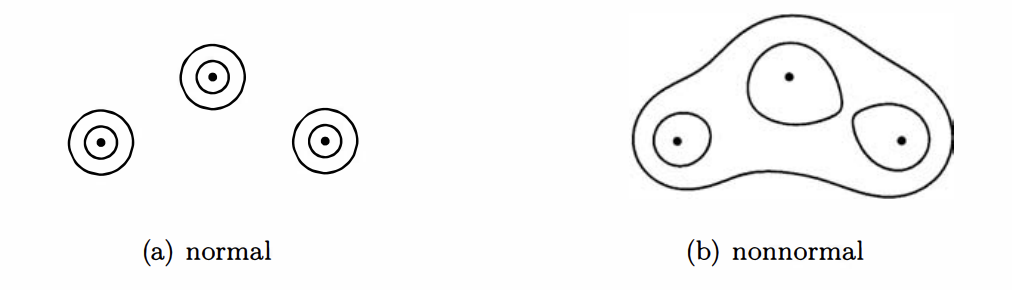
\includegraphics[width=1.0\linewidth]{normal_vs_nonormal.png}
    \caption{Comparing the $\epsilon$-pseudospectra of normal and nonormal matrices. In each plot, the contours represent the boundary of $\sigma_{\epsilon}(A)$ for two values of $\epsilon.$ This figure was adapted from \cite{Nick}.}
    \label{compare}
\end{figure}
%             \mid
%             \|(A-zI)v\| < \epsilon
%             \text{ for some } v \in \mathbb{C}^N
%             \text{ with } \|v\|=1
%             \right\}.
%         \]
%     \end{enumerate}
% \end{theorem}


When $A$ is normal, the $\epsilon$-pseudospectrum is the union of open $\epsilon$-balls about the point in the spectrum of $A.$ This behaviour is depicted in Figure \ref{compare}. Equivalently, the resolvent norm satisfies $\|(A-zI)^{-1}\| = 1 / \text{dist}(z, \sigma(A))$ \cite{Nick}. 

Before moving on to the pseudospectra of linear operators, we summarize some general properties of the $\epsilon$-pseudospectrum of $A$ in the following theorem:
\begin{theorem}[{Properties of pseudospectra \cite[Theorem 2.4]{Nick}}]
    Let $A\in \mathbb{C}^{N\times N}$ and $\epsilon>0$ be arbitrary.
    \begin{enumerate}
        \item $\sigma_\epsilon(A)$ is nonempty, open, and bounded, with at most $N$ connected components, each containing one or more eigenvalues of $A$.

        \item If $\|\cdot\|=\|\cdot\|_2$, then
        \[
            \sigma_\epsilon(A^*)=\overline{\sigma_\epsilon(A)}.
        \]

        \item If $\|\cdot\|=\|\cdot\|_2$, then
        \[
            \sigma_\epsilon(A_1\oplus A_2)
            =
            \sigma_\epsilon(A_1)\cup \sigma_\epsilon(A_2).
        \]

        \item For any $c\in\mathbb{C}$,
        \[
            \sigma_\epsilon(A+c)=c+\sigma_\epsilon(A).
        \]

        \item For any nonzero $c\in\mathbb{C}$,
        \[
            \sigma_{|c|\epsilon}(cA)=c\sigma_\epsilon(A).
        \]
    \end{enumerate}
\end{theorem}

\section{Pseudospectra of Linear Operators}

We now generalize these results to the case of linear operators. Let $X$ be a Banach space and $T \in C(X, X).$ The $\epsilon$-pseudospectrum of $T$ can be defined by any of the following three equivalent definitions:

\begin{definition}[{$\epsilon$-pseudospectrum \cite[4.3, 4.4, 4.5]{krey}}] \label{pseudo def}
    Let $X$ be a Banach space, $T\in C(X, X),$ and $\epsilon>0$ be arbitrary. The
    following definitions of $\epsilon$-pseudospectrum of $T$ are equivalent:
    \begin{enumerate}
        \item
            $\sigma_\epsilon(T)
            =
            \left\{
            z\in\mathbb{C}
            \mid
            \left\|R_T(z) \right\|>\epsilon^{-1}
            \right\}.$
        \item
            $\sigma_\epsilon(T)
            =
            \left\{
            z\in\mathbb{C}
            \mid
            z\in\sigma(T+E)
            \text{ for some } E\in\mathcal{B}(X)
            \text{ with } \|E\|<\epsilon
            \right\}.$
        \item $\sigma_\epsilon(T)
            =
            \left\{
            z\in\mathbb{C}
            \mid
            z\in\sigma(T)
            \text{ or }
            \|T_zu\|<\epsilon
            \text{ for some } u\in\mathcal{D}(T)
            \text{ with } \|u\|=1
            \right\}.$
    \end{enumerate}

    % If
    % \[
    %     \|(T-zI)u\|<\epsilon
    % \]
    % as in Definition $3$, then $z$ is called an $\epsilon$-pseudoeigenvalue of
    % $T$, and $u$ is called a corresponding $\epsilon$-pseudoeigenvector, or
    % pseudomode.
\end{definition}
Here, we adopt the convention that if $z \in \sigma(T),$ then $\| R_T(z) \| =\infty.$ Thus, the spectrum of $T$ is a subset of the $\epsilon$-pseudospectrum for all $\epsilon > 0.$ The complement of the $\epsilon$-pseudospectrum is called the \textit{$\epsilon$-pseudoresolvent.}

We summarize some key properties of the $\epsilon$-pseudospectrum of $T$ in the following theorem:
\begin{theorem}[{Properties of pseudospectra of $T$ \cite[Lecture 2]{umberto}}]
    Let $X$ be a Banach space and $T \in C(X, X).$ We have the following results:
    \begin{enumerate}[label=(\alph*)]
        \item If $\epsilon_1 > \epsilon_2 > 0,$ then $\sigma_{\epsilon_2}(T) \subset \sigma_{\epsilon_1}(T).$
    \item $\sigma(T) = \cap_{\epsilon > 0} \, \sigma_{\epsilon}(T).$
    \item Each connected component of $\sigma_{\epsilon}(T)$ has a nonempty intersection with $\sigma(T)$\footnote{Loosely speaking, the $\epsilon$-pseudospectrum does not form a detached `island' away from the true spectrum.}.
    \item $\sigma_{\epsilon}(T)$ is closed.
    \end{enumerate}
\end{theorem}
\begin{proof}
    Monotonicity, i.e., $\sigma_{\epsilon_2}(T) \subset \sigma_{\epsilon_1}(T),$ follows directly from the definition of the $\epsilon$-pseudospectrum. In particular, if $\epsilon_1 > \epsilon_2,$ then $\|R_T(z) \| > \epsilon_2^{-1}$ implies $\|R_T(z) \| > \epsilon_1^{-1}.$

    If $z \in \sigma(T),$ then $z \in \sigma_{\epsilon}(T)$ for all $\epsilon > 0.$ If $z \in \rho(T)$ then $\| R_T(z) \| < \infty.$ Thus, we can find some $\epsilon > 0$ such that $\| R_T(z) \| \le 1/\epsilon,$ in which $z$ is in the $\epsilon$-pseudoresolvent of $T.$ Consequently, as $\epsilon$ decreases, each $z \in \rho(T)$ is eventually excluded from the $\epsilon$-pseudospectrum. Thus, $\sigma(T) = \cap_{\epsilon > 0} \, \sigma_{\epsilon}(T).$

    For the sake of contradiction, suppose that $\mathcal{C}$ is a connected component of $\sigma_{\epsilon}(T)$ such that $\mathcal{C} \cap \sigma(T) = \emptyset.$ Then $\mathcal{C} \subset \rho(T)$ and $R_T(z)$ is analytic on $\mathcal{C}.$ In this case, the scalar function $z \rightarrow \| R_T(z) \|$ is a subharmonic function on $\mathcal{C}$ \cite{umberto}. In the interior of $\mathcal{C},$ $z$ is in the $\epsilon$-pseudospectrum of $T$ and $\| R_T(z) \| > \epsilon^{-1}.$ On the boundary of $\mathcal{C},$ $\| R_T(z) \| = \epsilon^{-1}.$ Thus, $\| R_T(z) \|$ is strictly larger in the interior of $\mathcal{C}$ than on its boundary. This contradicts the maximum principle for subharmonic functions\footnote{Subharmonic functions follow a maximum principle, where they cannot have a strict maximum in the interior of their domain unless they are constant.}. Thus, $\mathcal{C} \cap \sigma(T) \ne \emptyset.$

    \end{proof}

As indicated by Figure \ref{compare}, when an operator is compact and normal, the $\sigma_{\epsilon}(T)$ is the union of open disks of radius $\epsilon,$ centered at each point in $\sigma(T).$ This observation is formalized in the following theorem:
\begin{theorem}
    Let $H$ be a separable Hilbert space and $T \in K(H, H)$ be normal. Then 
    \begin{equation}
        \sigma_{\epsilon}(T) = \{ z \in \mathbb{C} \mid \text{dist}(z, \sigma(T)) < \epsilon \}.
    \end{equation}
\end{theorem}
\begin{proof}
    Since $T$ is compact and normal, Theorem \ref{HB} tells us that we can find a Hilbert basis of $H$ comprised of the eigenvectors of $T.$ Denote this basis $\{h_n \}_{n \in \mathbb{N}}$ with corresponding eigenvalues $\{z_n\}_{n \in \mathbb{N}}.$ Consider $h \in H,$ which we can write as 
    \begin{equation}
        h = \sum_{n \in \mathbb{N}} (h, h_n)_H h_n.
    \end{equation}
    % Then, 
    % \begin{equation}
    %       T_z h = \sum_{n \in \mathbb{N}} (z_n - z) (h, h_n)_H h_n.
    % \end{equation}
    Consider $z \in \rho(T).$ Then $R_T(z) \,h =  \sum_{n \in \mathbb{N}} (z_n - z)^{-1} (h, h_N)_H h_n.$ Thus, 
    \begin{equation}
        \| R_T(z) \| = \sup_{n \in \mathbb{N}} \frac{1}{|z_n - z|} = \frac{1}{\text{dist}(z, \sigma(T))}.
     \end{equation}
     Consequently, $\| R_T(z) \| > \epsilon^{-1} $ if and only if $\text{dist}(z, \sigma(T)) < \epsilon,$ as desired.
\end{proof}


Similar to the finite-dimensional case, the pseudopectra of $T$ can be used to explore stability. Consider solving $T_z x = y.$ If $z \in \rho(T),$ then $x = R_T(z) y$  and $\|x \| \le \|R_T(z) \| \| y \|.$ 
If $T$ is a compact and normal operator, $\| R_T(z) \| = \text{dist}(z, \sigma(T))^{-1}.$ Thus, $\| x \| \le \text{dist}(z, \sigma(T))^{-1} \|y \|.$ This is a statement about the stability in solving $T_z x = y,$  with perturbations in $y$ producing changes in $x$ that are at most
$\text{dist}(z,\sigma(T))^{-1}$ times as large.

The situation is very different for nonnormal operators, where we only have that $\| R_T(z) \| \ge 1 / \text{dist}(z, \sigma(T)).$ This lack of control indicates the potential for instability. To characterize this instability, we may study the $\epsilon$-pseudospectra of $T.$ 
In particular, if we demand $\| R_T(z) \| \le \epsilon^{-1},$ we obtain $\| x \| \le \epsilon^{-1} \| y \|.$ Thus, we can think of the $\epsilon$-pseudoresolvent as the set of $z$ for which the problem $T_z x  = y$ is stable, with perturbations in $y$ producing changes in $x$ that are at most
$\epsilon^{-1}$ times as large.




As expected, we can use the $\epsilon$-pseudospectrum to define $\epsilon$-eigenvalues and $\epsilon$-eigenvectos of $T.$ 

\begin{definition}[$\epsilon$-eigenvalues and $\epsilon$-eigenvectors]
    Let $X$ be a Banach space, $T \in C(X, X),$ and $\epsilon > 0$ be arbitary.  
    A $z \in \mathbb{C}$ is called an $\epsilon$-eigenvalue of $T$ if there exists an $x \in X$ such that $\|x\| = 1$ and 
    \begin{equation}
       \|T_z \, x \| < \epsilon
    \end{equation}
    The corresponding $x$ are $\epsilon$-eigenfunctions of $T$ corresponding to $z.$ 
    The set of all $\epsilon$-eigenvalues of $T$ is denoted $\Gamma_{\epsilon}(T).$
\end{definition}

When $z$ is an eigenvalue of $T$ then $\|T_z \, x \| = 0 < \epsilon.$ Thus, $\Gamma(T) \subset \Gamma_{\epsilon}(T).$ Furthermore, the third definition of $\sigma_{\epsilon}(T)$ in Definition \ref{pseudo def} shows that every $\epsilon$-eigenvalue of $T$ is in $\sigma_{\epsilon}(T),$ Therefore, $\Gamma_{\epsilon}(T) \subset \sigma_{\epsilon}(T).$




% Thus the subharmonic function $\|R_T(z)\|$ is strictly larger in the interior of
% $\mathcal C$ than on the boundary. This contradicts the maximum principle for
% subharmonic functions, which implies that a subharmonic function cannot have
% interior values strictly exceeding its boundary supremum


\newpage
\bibliographystyle{plainurl}
\bibliography{background}

\end{document}
